\chapter[RESULTADOS]{RESULTADOS}

\section{Malha em formato 'L'}
Conforme já especificado, a malha a ser resolvida para o problema de difusão de calor 2D é uma malha em formato 'L'. Tal malha, gerada por uma triangulação de Delaunay em um domínio fechado é apresentada na figura \ref{fig:malha-inicial}.

Nessa malha aparecem em todos as células o valor da solução analítica seguido do valor numérico encontrado. Em vermelho estão os centroides dos volumes 'Reais' e em azul o centroide dos volumes 'Virtuais'

Além de visualizar a malha, é muito útil a informação de maior ângulo, menor ângulo, desvio padrão do ângulo, média da qualidade da malha, maior qualidade, menor qualidade resultando nas tabelas \ref{tab:angulos-malha-inicial} e \ref{tab:qualidades-malha-inicial}. As qualidades se referem às qualidades de cada volume que constitui a malha, sendo que esta é obtida pela fórmula:

\begin{equation}
    2 \frac{r}{R}
    \label{eq:qualidade}
\end{equation}

Onde $r$ é o raio da circunferência inscrita e $R$ é o raio da circunferência circunscrita.
\criarsimbolo{$r$}{raio daa circunferência inscrita}
\criarsimbolo{$R$}{raio daa circunferência circunscrita}

A média das qualidades pode ser associada à malha como uma indicação da sua qualidade geral.

De modo a testar os algoritmos de suavização da malha, esta malha inicial foi distorcida, ou seja, seus vértices internos foram propositalmente alterados de posição, resultando na malha \ref{fig:malha-ruim} com as tabelas \ref{tab:angulos-malha-distorcida} e \ref{tab:qualidades-malha-distorcida}.

\newpage
\subsection{Malha Inicial}

\begin{figure}[ht]
    \centering
    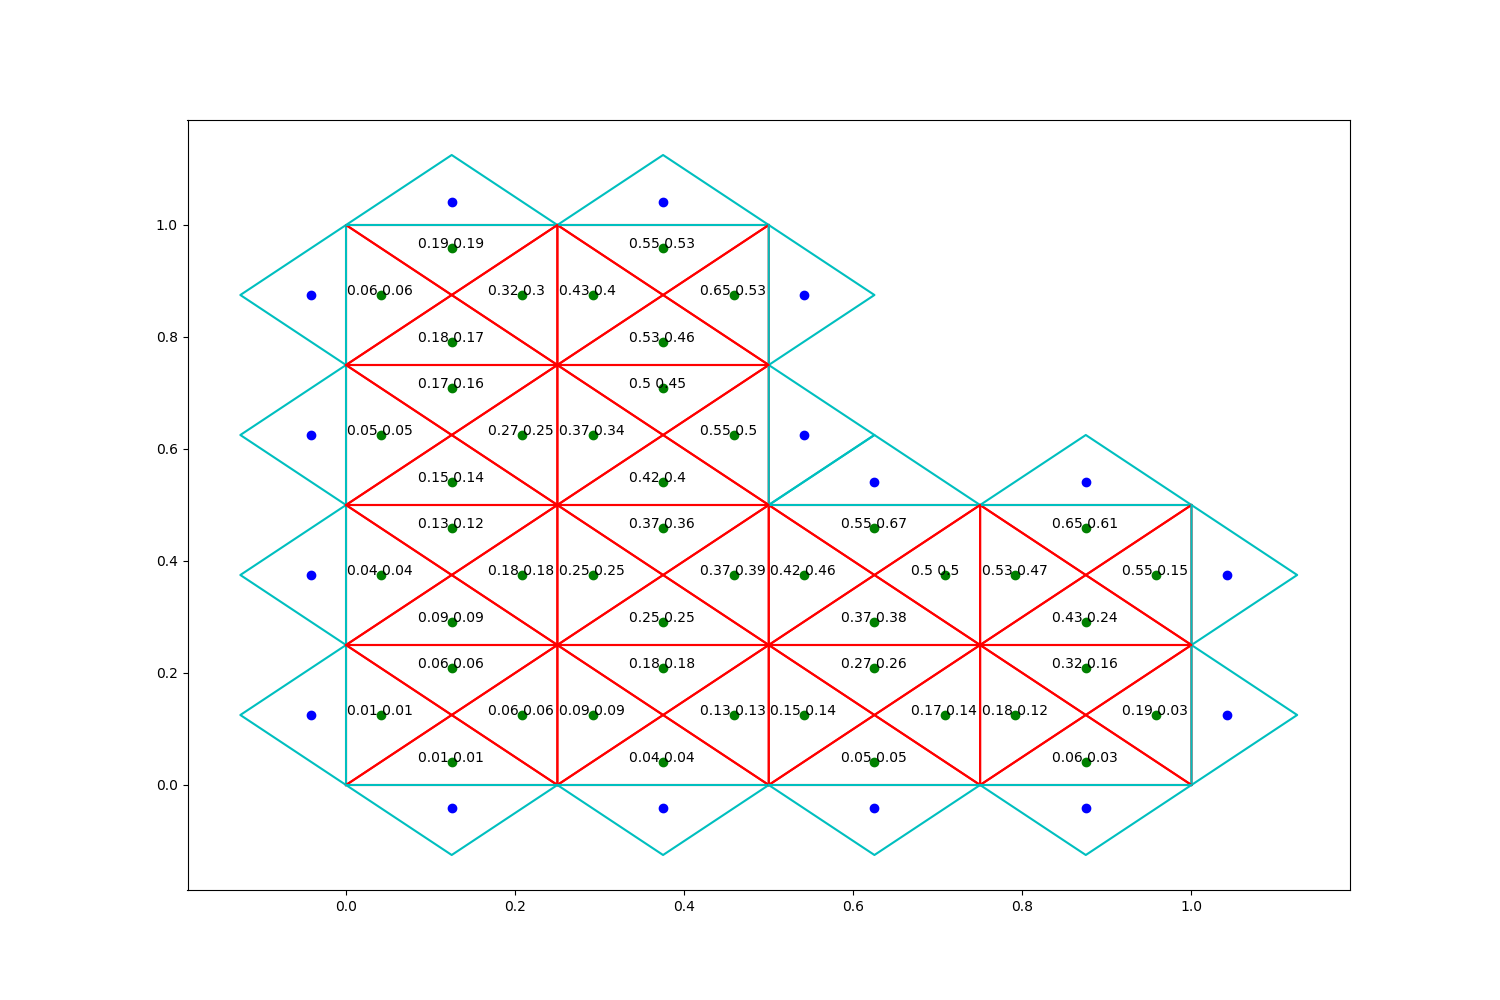
\includegraphics[width=1\linewidth]{fig/malha_inicial.png}
    \caption{Malha Inicial}
    \label{fig:malha-inicial}
\end{figure}

Na tabela \ref{tab:angulos-malha-inicial} a seguir, temos os seguintes resultados:

\begin{enumerate}
    \item Maior: Maior ângulo interno dentre todas as triangulações criadas;
    \item Menor: Menor ângulo interno dentre todas as triangulações criadas;
    \item Média: A média entre os ângulos internos de todas as triangulações, como a soma dos ângulos internos de um triângulo é sempre 180 graus, essa média é sempre 60;
    \item Desvio Padrão: O valor do desvio padrão entre os valores dos ângulos internos, quanto menor esse valor mais próximos são os valores dos ângulos e portanto mais equiláteros são os triângulos.
\end{enumerate}

\begin{table}[hb]
 \centering
 \par\caption{Ângulos da Malha Inicial}
\begin{tabular}{c|c|c|c}
 Maior&menor&média&desvio padrão\\\hline\hline
  90&45&60&21.268663\\\hline
 \end{tabular}
 \label{tab:angulos-malha-inicial}
\end{table}

Já na tabela \ref{tab:qualidades-malha-inicial} temos os seguintes resultados:

\begin{enumerate}
    \item Maior: O maior valor encontrado entre os triângulos gerados para a equação \ref{eq:qualidade};
    \item Menor: O menor valor encontrado entre os triângulos gerados para a equação \ref{eq:qualidade};
    \item Média: A média da qualidade de todos os volumes;
    \item Desvio padrão: O desvio padrão da qualidade das malhas;
\end{enumerate}

\begin{table}[h!]
 \centering
 \par\caption{Qualidades da Malha Inicial}
\begin{tabular}{c|c|c|c}
 Maior&menor&média&desvio padrão\\\hline\hline
 8.284271e-01&8.284271e-01&8.284271e-01&0\\\hline
 \end{tabular}
 \label{tab:qualidades-malha-inicial}
\end{table}

\newpage
\subsection{Malha Distorcida}

\begin{figure}[ht]
    \centering
    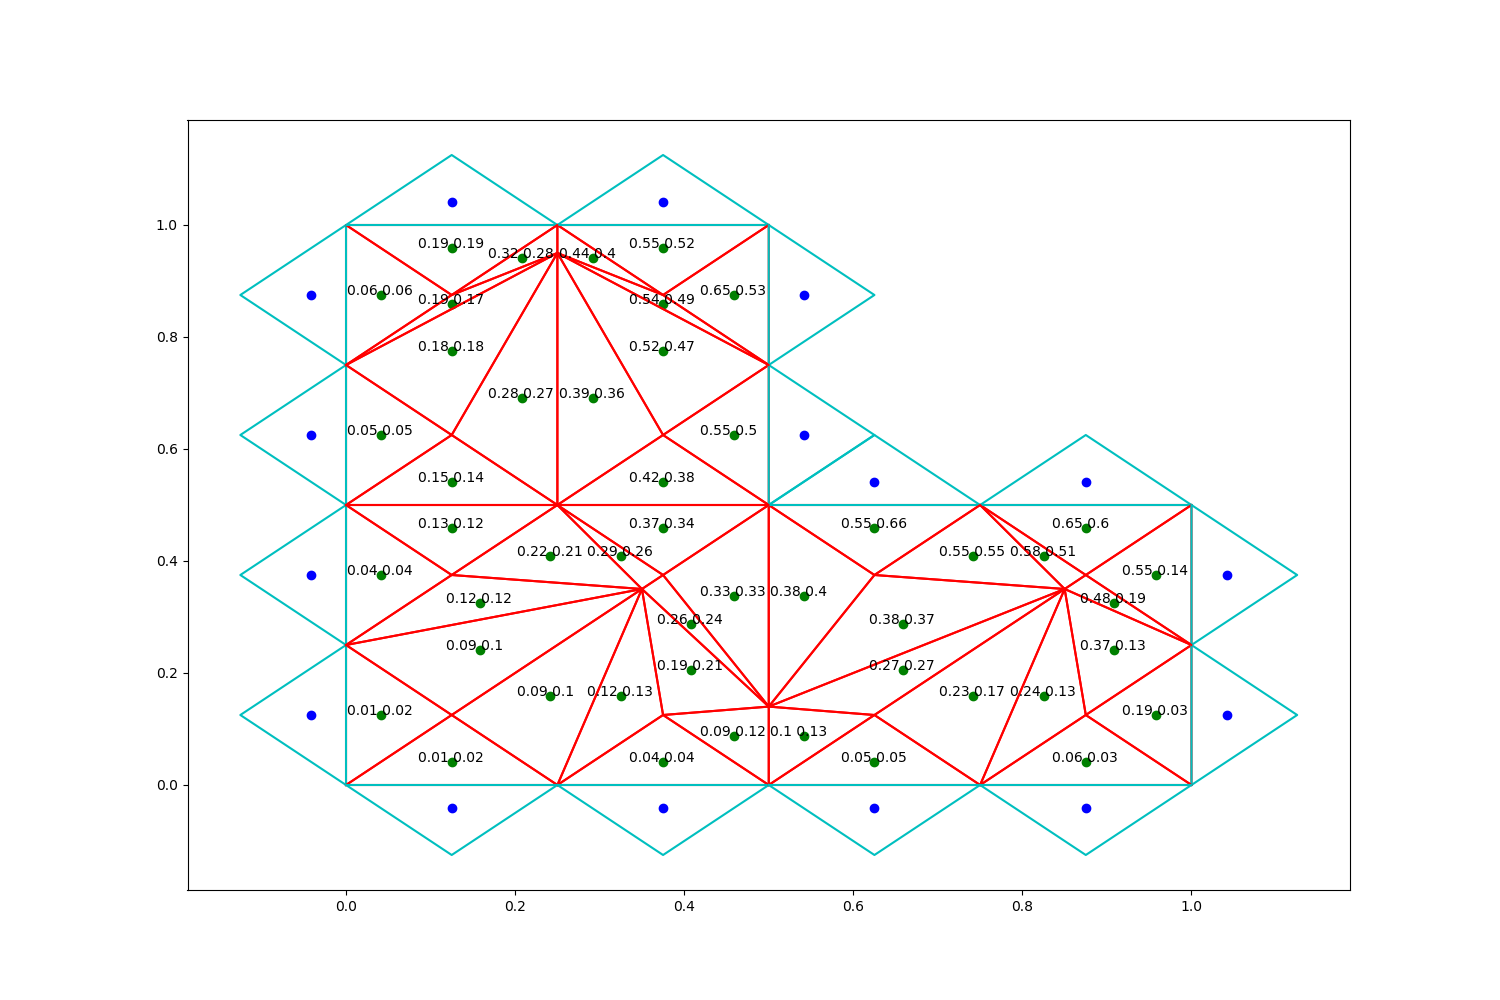
\includegraphics[width=1\linewidth]{fig/malha-ruim.png}
    \caption{Malha Inicial após Deformações}
    \label{fig:malha-ruim}
\end{figure}

Essa malha foi propositalmente distorcida de modo a se poder comparar os algoritmos de suavização. Como pode ser visto na tabela \ref{tab:angulos-malha-distorcida} o maior ângulo encontrado aumentou e o menor diminuiu. A média das qualidade de malha, que é usada como métrica da qualidade, diminuiu de valor.

\begin{table}[hb]
\centering
\par\caption{Ângulos da Malha Distorcida}
\begin{tabular}{c|c|c|c}
Maior&menor&média&desvio padrão\\\hline\hline
165.963757&6.340192&60.000000&30.017315\\\hline
\end{tabular}
\label{tab:angulos-malha-distorcida}
\end{table}



\begin{table}[hb]
\centering
\par\caption{Qualidades da Malha Distorcida}
\begin{tabular}{c|c|c|c}
Maior&menor&média&desvio padrão\\\hline\hline
0.928007&0.029467&0.700351&0.227835\\\hline
\end{tabular}
\label{tab:qualidades-malha-distorcida}
\end{table}

\newpage
\subsection{Centroidal Path Tesselation}

Em seguida, executou-se os algoritmos de melhoramento da malha com apenas uma iteração, começando pelo método centroidal patch tesselation (CPT) como na figura \ref{fig:malha-cpt}

\begin{figure}[ht]
    \centering
    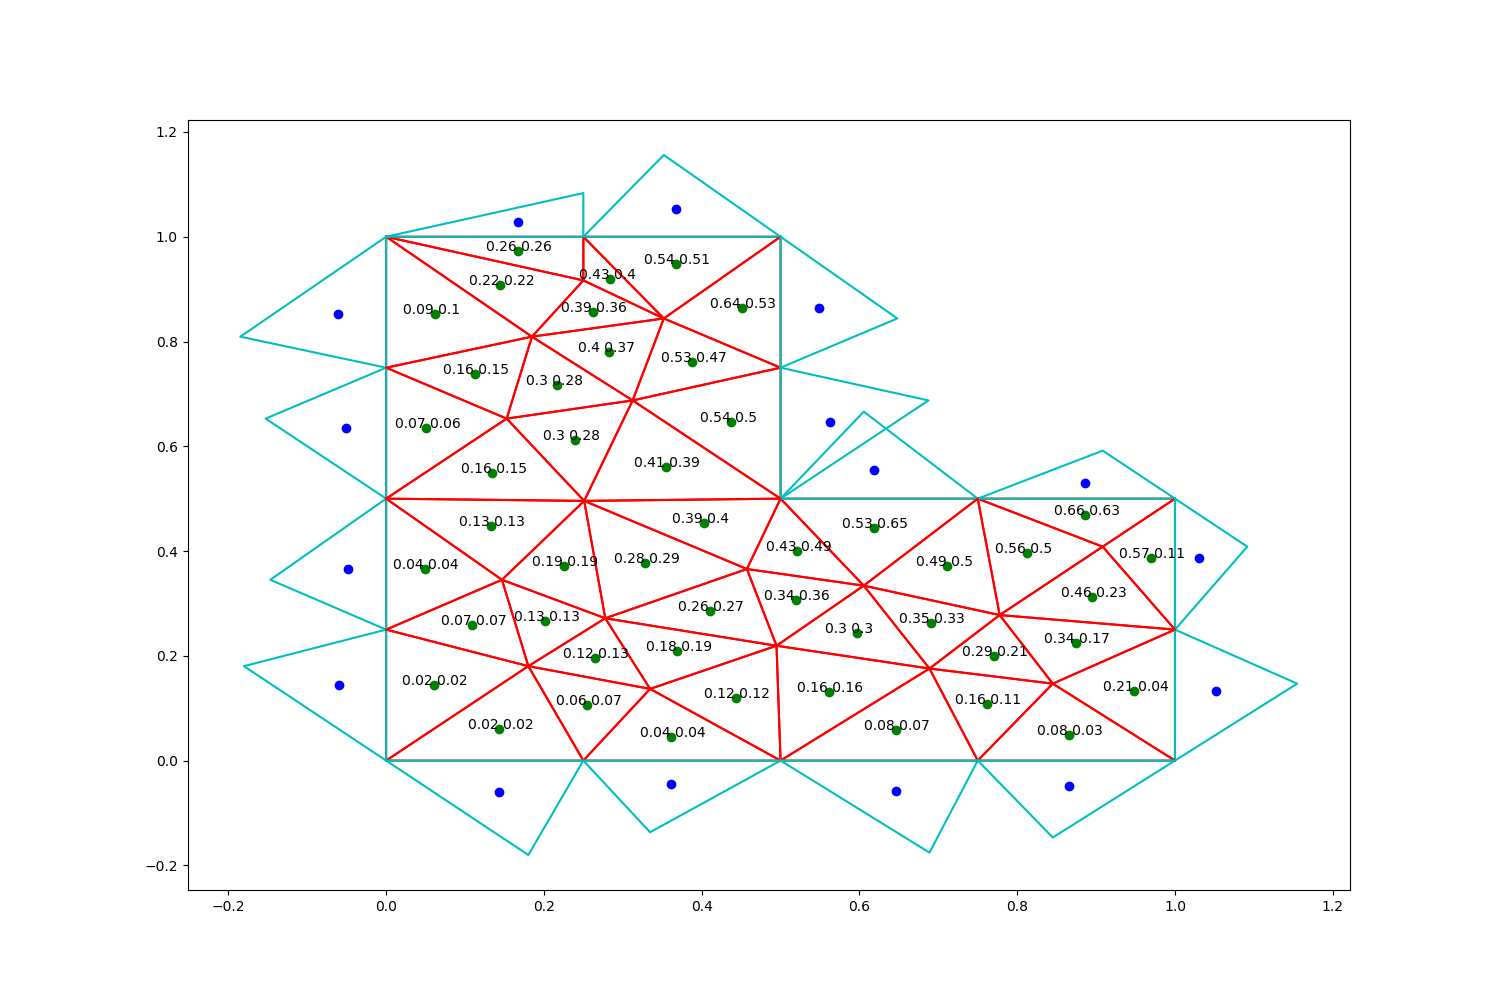
\includegraphics[width=1\linewidth]{fig/malha-cpt.png}
    \caption{Melhoramento CPT}
    \label{fig:malha-cpt}
\end{figure}

Pode-se observar que a média da qualidade aumentou de valor com essa suavização.

\begin{table}[hb]
\centering
\par\caption{Ângulos da Malha CPT}
\begin{tabular}{c|c|c|c}
Maior&menor&média&desvio padrão\\\hline\hline
121.713423&28.467019&60.000000&16.206878\\\hline
\end{tabular}
\label{tab:angulos-malha-cpt}
\end{table}

\begin{table}[hb]
\centering
\par\caption{Qualidades da Malha CPT}
\begin{tabular}{c|c|c|c}
Maior&menor&média&desvio padrão\\\hline\hline
0.999109&0.582970&0.919103&0.086327	\\\hline
\end{tabular}
\label{tab:qualidades-malha-cpt}
\end{table}

\newpage
\subsection{Optimal Delaunay Tesselation}

\begin{figure}[ht]
    \centering
    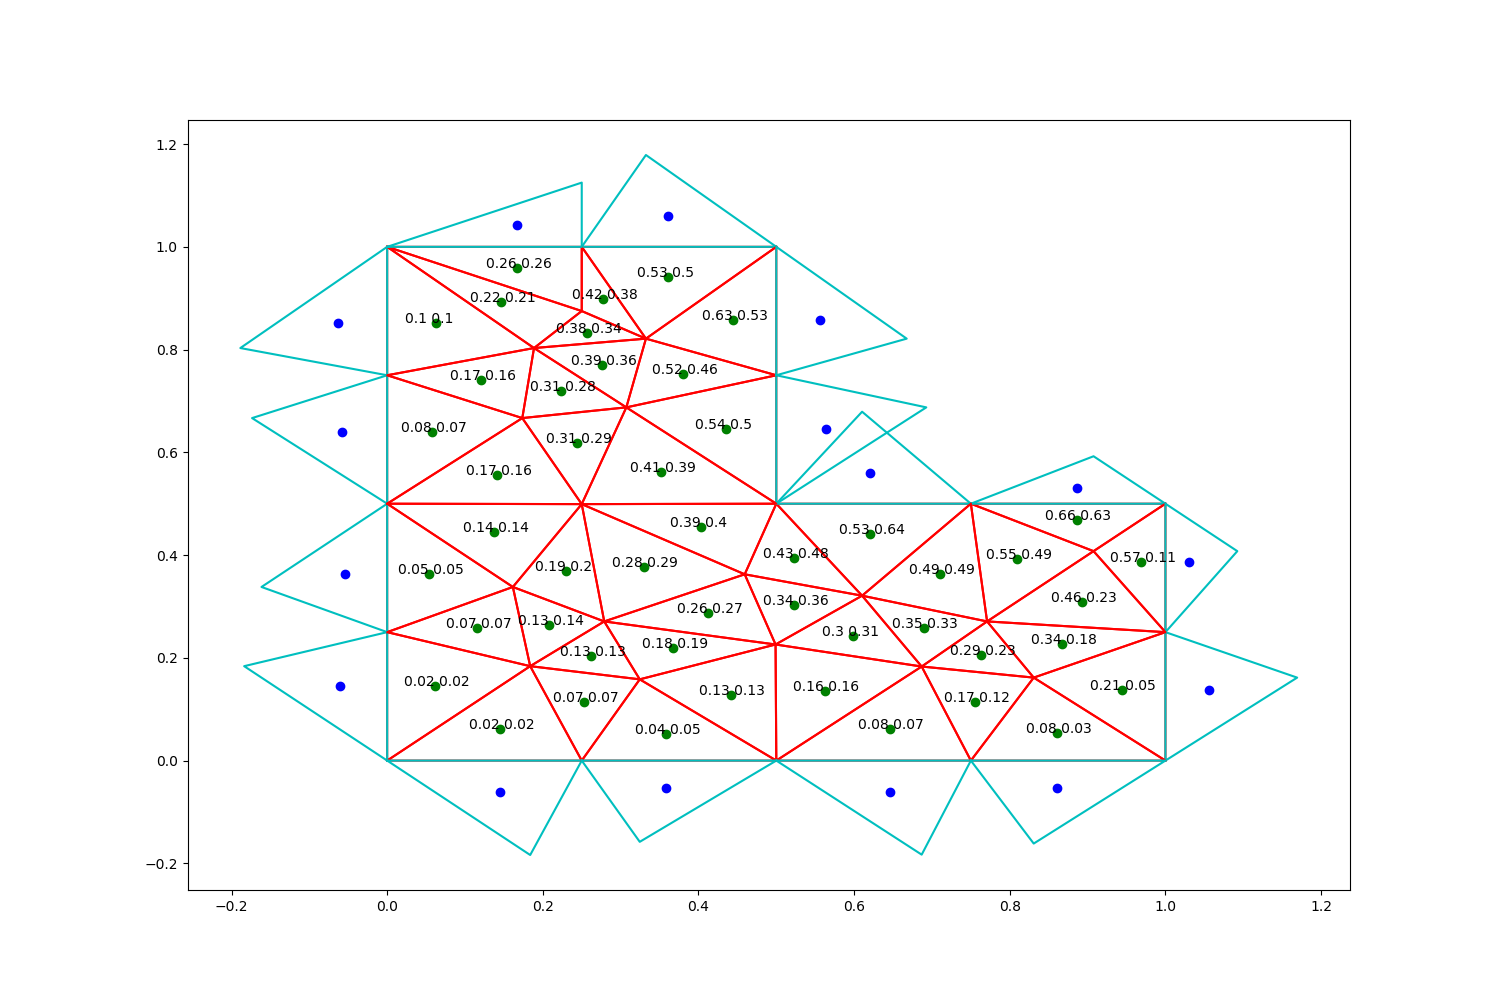
\includegraphics[width=1\linewidth]{fig/malha-odt.png}
    \caption{Melhoramento ODT}
    \label{fig:malha-odt}
\end{figure}

Esse algoritmo também apresentou um valor de média de qualidade superior em relação a malha original.

\begin{table}[hb]
\centering
\par\caption{Ângulos da Malha ODT}
\begin{tabular}{c|c|c|c}
Maior&menor&média&desvio padrão\\\hline\hline
92.339656&36.765310&60.000000&14.499022\\\hline
\end{tabular}
\label{tab:angulos-malha-odt}
\end{table}

\begin{table}[hb]
\centering
\par\caption{Qualidades da Malha ODT}
\begin{tabular}{c|c|c|c}
Maior&menor&média&desvio padrão\\\hline\hline
0.997704&0.823047&0.926443&0.046574\\\hline
\end{tabular}
\label{tab:qualidades-malha-odt}
\end{table}

\newpage
\subsection{Centroidal Voronoi Tesselation}

\begin{figure}[ht]
    \centering
    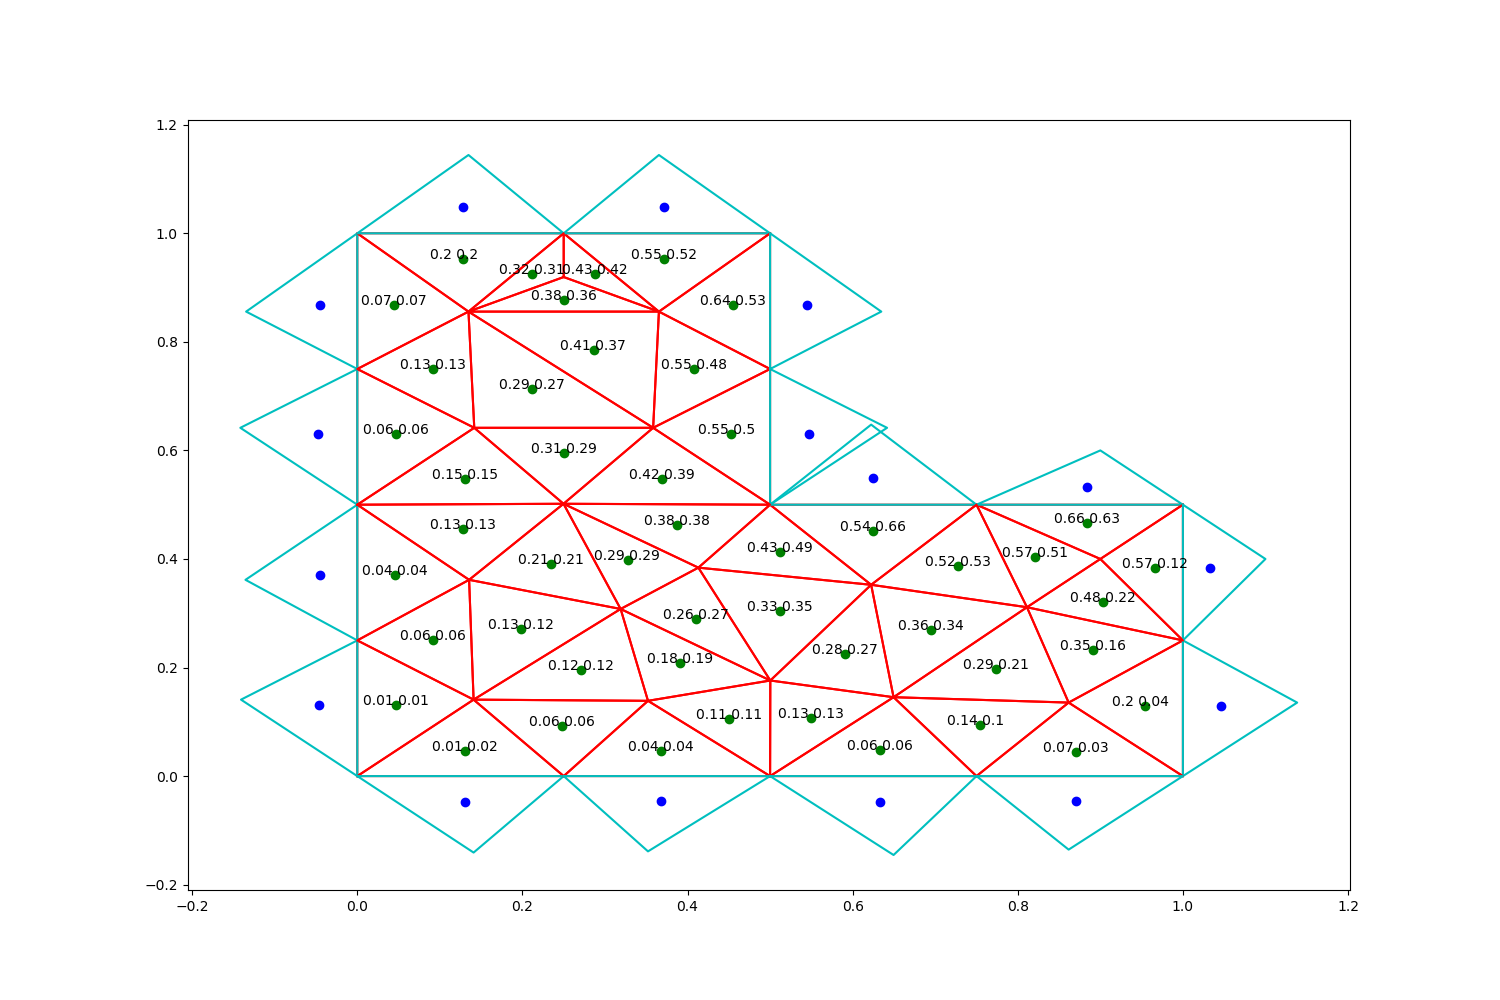
\includegraphics[width=1\linewidth]{fig/malha-cvt.png}
    \caption{Melhoramento CVT}
    \label{fig:malha-cvt}
\end{figure}

O CVT apresentou valores semelhantes aos outros algoritmos para a malha usada.

\begin{table}[hb]
\centering
\par\caption{Ângulos da Malha CVT}
\begin{tabular}{c|c|c|c}
Maior&menor&média&desvio padrão\\\hline\hline
98.568632&36.794950	&60.000000&17.275253\\\hline
\end{tabular}
\label{tab:angulos-malha-cvt}
\end{table}

\begin{table}[hb]
\centering
\par\caption{Qualidades da Malha CVT}
\begin{tabular}{c|c|c|c}
Maior&menor&média&desvio padrão\\\hline\hline
0.990750&0.787629&0.907101&0.059118\\\hline
\end{tabular}
\label{tab:qualidades-malha-cvt}
\end{table}

\newpage
\subsection{Angle Based Tesselation}

\begin{figure}[ht]
    \centering
    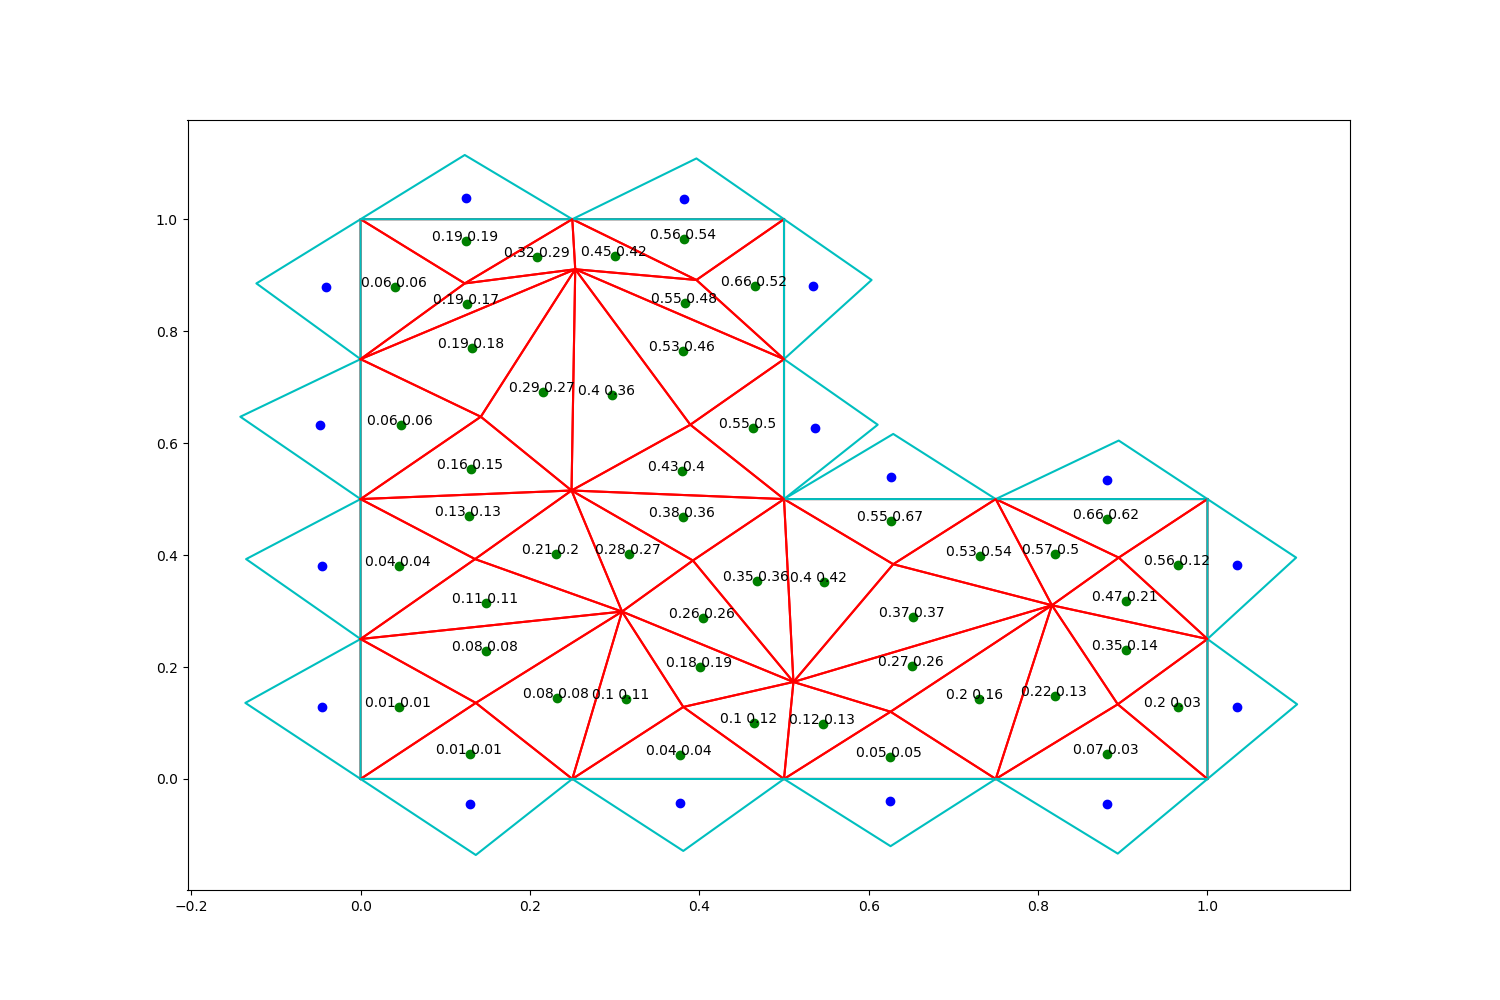
\includegraphics[width=1\linewidth]{fig/malha-angulos.png}
    \caption{Melhoramento Ângulos}
    \label{fig:malha-angulos}
\end{figure}

O algoritmo ABT resultou em uma qualidade inferior com relação aos outros métodos.

\begin{table}[hb]
\centering
\par\caption{Ângulos da Malha Ângulos}
\begin{tabular}{c|c|c|c}
Maior&menor&média&desvio padrão\\\hline\hline
90.003446	&44.996564&60.000000&21.268508\\\hline
\end{tabular}
\label{tab:angulos-malha-angulos}
\end{table}

\begin{table}[hb]
\centering
\par\caption{Qualidades da Malha Ângulos}
\begin{tabular}{c|c|c|c}
Maior&menor&média&desvio padrão\\\hline\hline
0.866070&0.865999&0.866027	&0.000013\\\hline
\end{tabular}
\label{tab:qualidades-malha-angulos}
\end{table}

\newpage
\subsection{Gurobi Optimization Based Tesselation}

\begin{figure}[ht]
    \centering
    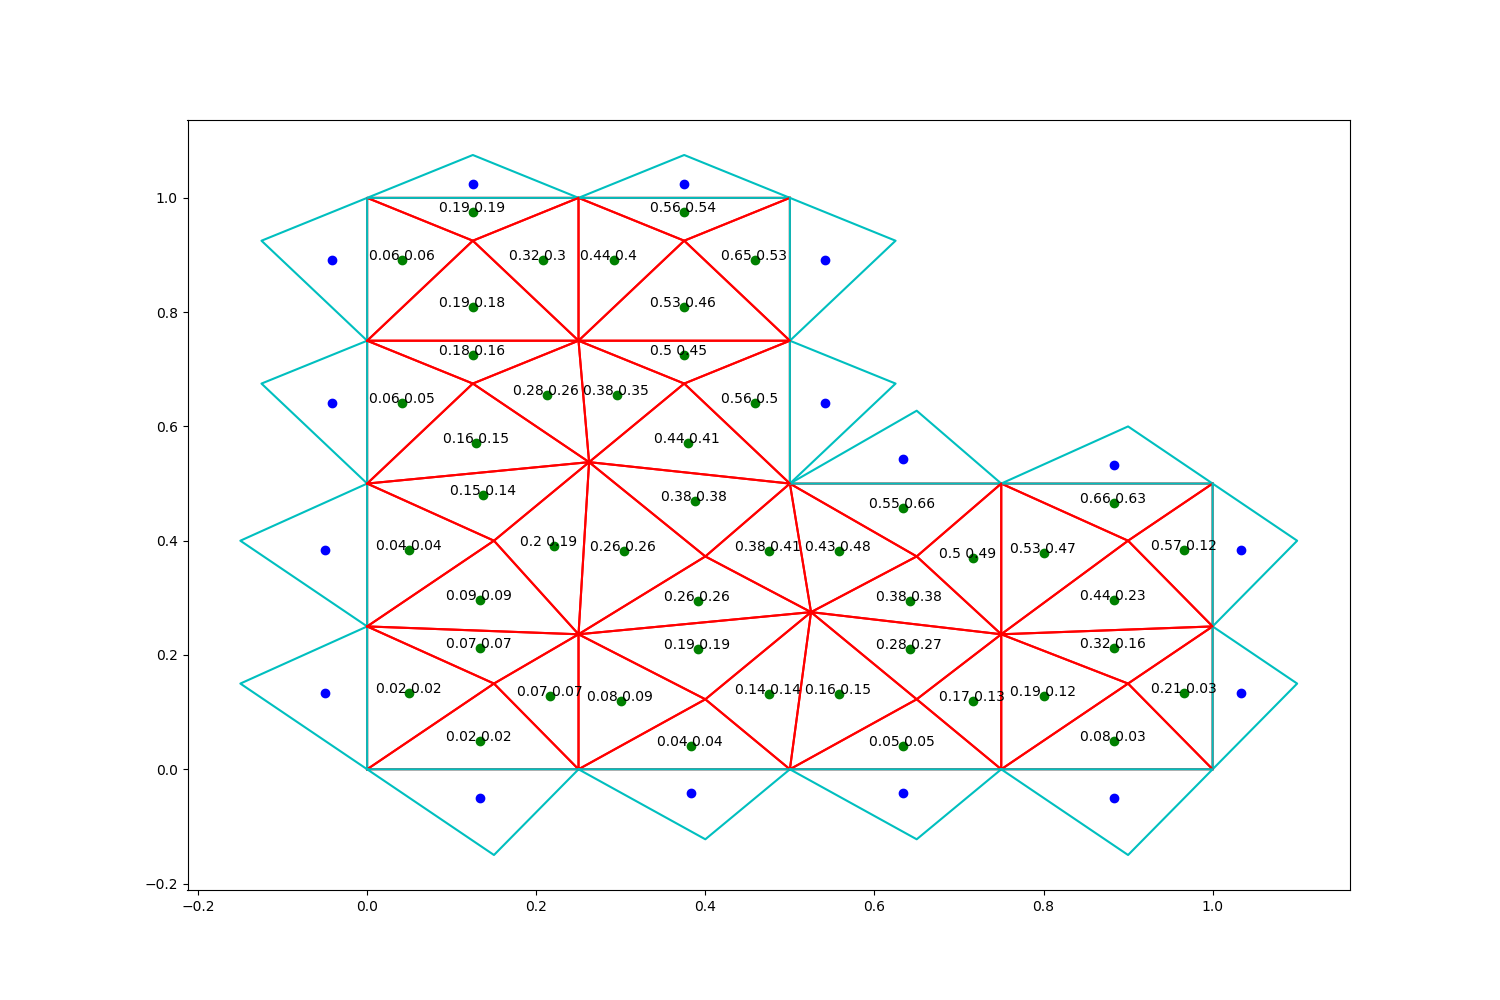
\includegraphics[width=1\linewidth]{fig/malha-gurobi.png}
    \caption{Melhoramento Gurobi}
    \label{fig:malha-gurobi}
\end{figure}

O método de suavização baseado em otimização usando-se o Gurobi resultou um valor de qualidade ligeiramente inferior, no entanto, tal resultado pode ser atribuído ao fato do modelo linear adotado usar como meta a minimização de todos os ângulos internos dos triângulos. Também deve-se levar em consideração que para uma malha maior o tempo computacional aumentaria bastante em relação aos outros métodos vistos até agora.

\begin{table}[hb]
\centering
\par\caption{Ângulos da Malha Gurobi}
\begin{tabular}{c|c|c|c}
Maior&menor&média&desvio padrão\\\hline\hline
118.072487	&30.541971&60.000000&24.045397\\\hline
\end{tabular}
\label{tab:angulos-malha-gurobi}
\end{table}

\begin{table}[hb]
\centering
\par\caption{Qualidades da Malha Gurobi}
\begin{tabular}{c|c|c|c}
Maior&menor&média&desvio padrão\\\hline\hline
0.977771&0.618590&0.831586&0.098368\\\hline
\end{tabular}
\label{tab:qualidades-malha-gurobi}
\end{table}

\newpage
\subsection{Genetic Algorithm Based Tesselation}

\begin{figure}[ht]
    \centering
    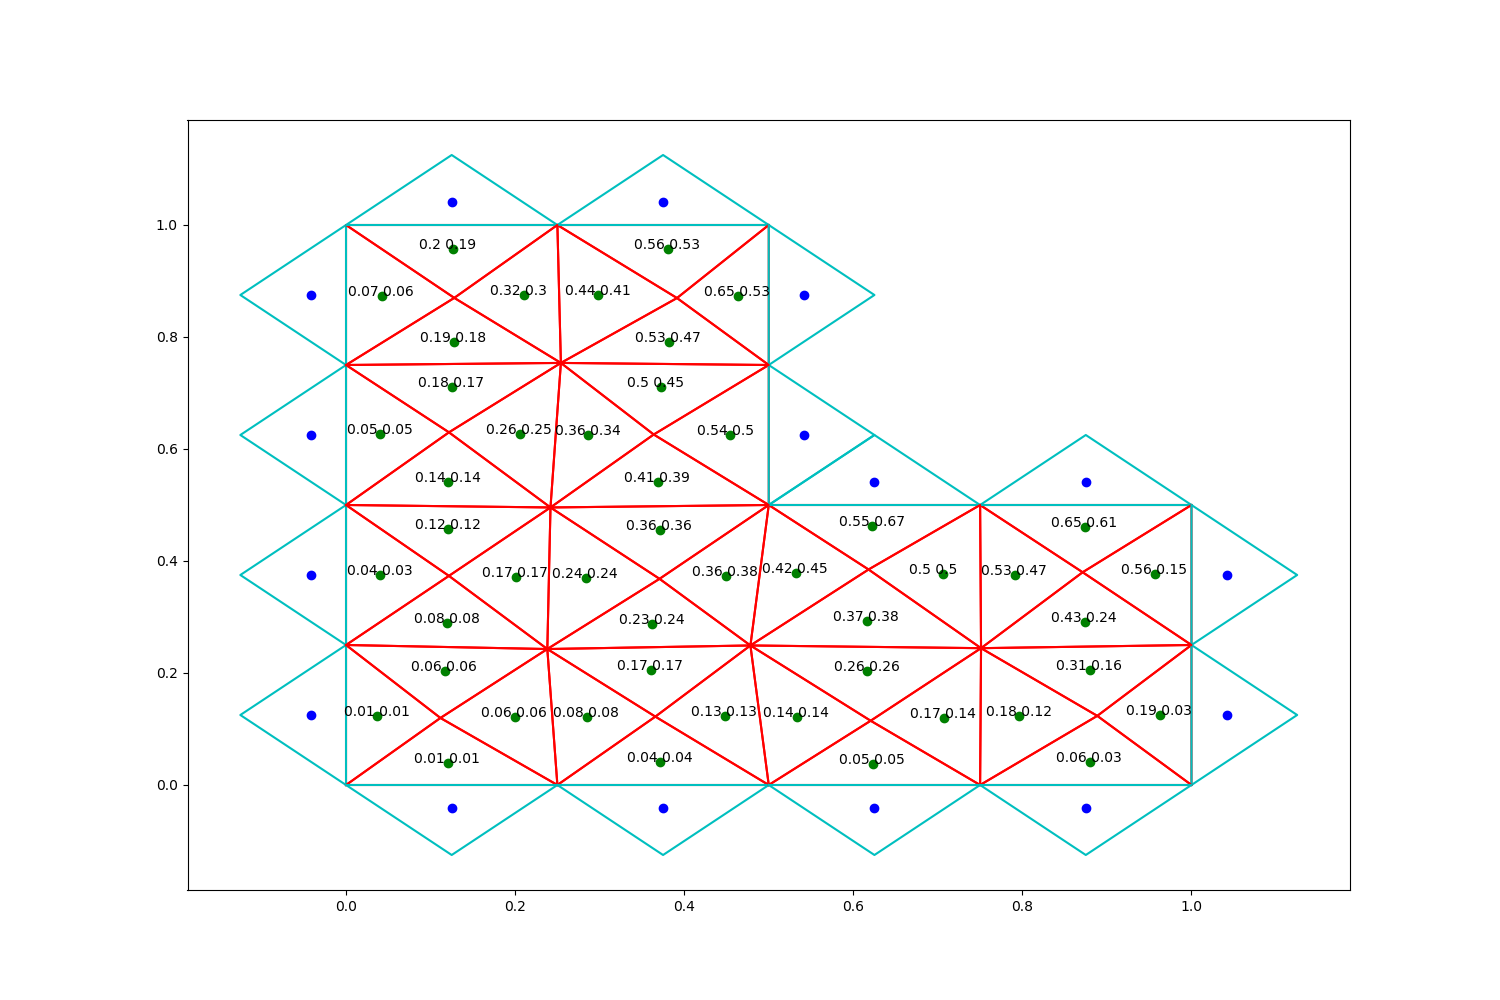
\includegraphics[width=1\linewidth]{fig/malha-ga.png}
    \caption{Melhoramento GA}
    \label{fig:malha-ga}
\end{figure}

O método de suavização baseado no algoritmo genético resultou em um bom valor para a qualidade da malha, no entanto, a média da qualidade dos seus volumes foi inferior aos outros métodos.

\begin{table}[hb]
\centering
\par\caption{Ângulos da Malha GA}
\begin{tabular}{c|c|c|c}
Maior&menor&média&desvio padrão\\\hline\hline
103.651693&36.916308&60.000000&21.561762\\\hline
\end{tabular}
\label{tab:angulos-malha-ga}
\end{table}

\begin{table}[hb]
\centering
\par\caption{Qualidades da Malha GA}
\begin{tabular}{c|c|c|c}
Maior&menor&média&desvio padrão\\\hline\hline
0.924401&0.751680&0.862425&0.033582\\\hline
\end{tabular}
\label{tab:qualidades-malha-ga}
\end{table}

\section{Comparação entre os algorítmos}

Na tabela \ref{tab:comparacao-analitico} está o valor da média das diferenças entre o valor analítico e numérico para todos os algorítmos usados no trabalho em ordem crescente, ou seja, por essa métrica o algorítmo de melhoramento por ângulos e o genético foram os melhores.

\begin{table}
    \centering
    \par\caption{Comparação entre as médias das diferenças em relação ao valor analítico}
    \begin{tabular}{c|c}
        Algoritmo&diferença\\\hline\hline
        Ângulos  &  0.054529 \\\hline
        Genético &  0.054563 \\\hline
        Gurobi   &  0.056215 \\\hline
        CPT      &  0.060670 \\\hline
        ODT      &  0.060929 \\\hline
        CVT      &  0.062826 \\\hline
    \end{tabular}
    \label{tab:comparacao-analitico}
\end{table}

Já na tabela \ref{tab:comparacao-qualidade} temos a métrica da média das qualidades conforme foi definido. Nesse caso o melhor algoritmo foi o ODT.

\begin{table}
    \centering
    \par\caption{Comparação entre as médias qualidades dos volumes de controle}
    \begin{tabular}{c|c}
        Algoritmo&diferença\\\hline\hline
        ODT      &  0.926443 \\\hline
        CPT      &  0.919103 \\\hline
        CVT      &  0.907101 \\\hline
        Ângulos  &  0.866027 \\\hline
        Genético &  0.860447 \\\hline
        Gurobi   &  0.831586 \\\hline
    \end{tabular}
    \label{tab:comparacao-qualidade}
\end{table}